\documentclass[a4paper,12pt,fonts]{./tulpackage/tularticle}

% Zvetseni radkovani
\linespread{1.3}

% Vlastní seznamy s enumitem
\usepackage{enumitem}
\newlist{itemize*}{itemize}{2}
\setlist[itemize*]{itemsep=3pt, parsep=3pt, label=$\bullet$}
\setlist[itemize*,2]{label={--}}

% Mezery mezi odstavci misto odrazeni prvnich radku
\usepackage{parskip}
% Nastaveni sazby a zalamovani textu
\sloppy
\lefthyphenmin=2
\righthyphenmin=3
\hyphenpenalty=5000
\tolerance=1500
\emergencystretch=3.5em
\hbadness=2000
% Penalizace osamocených řádků
\widowpenalty=10000
\clubpenalty=10000
% Definice pomocneho prikazu pro ukazky
\newcommand{\cmddemo}[1]{\bigskip\parbox[c]{3.9cm}{\cmd{#1}}\parbox[c]{10cm}{\csname #1\endcsname}\bigskip}

% Lepší tabulky
\usepackage{booktabs}

% Správa bibliografie s biber
\usepackage[backend=biber]{biblatex}
\addbibresource{bibliography/example-tularticle-references.bib}

% Nastavení jazyka dokumentu na cestinu
\usepackage{polyglossia}
\setdefaultlanguage{czech}

% Popisky bez textu "Obrazek 1:" apod.
\usepackage{caption}
\captionsetup[figure]{labelformat=empty}
\captionsetup[table]{labelformat=empty}

% Nazev PDF v ramci metadat
\hypersetup{pdftitle={TU v Liberci (Příkladový článek)}}

% Uzivatelske informace
\newcommand{\doctitle}{TU v Liberci \newline(Příkladový článek)}
\newcommand{\name}{Ondřej Wiener}
\newcommand{\phone}{ Tel: neuvedeno}
\newcommand{\mail}{ondrej.wiener@tul.cz}
\newcommand{\location}{Liberec 2025}

% Predani informaci sablone
\TULname{\name}
\TULphone{\phone}
\TULmail{\mail}

% Prikazy specificke pro dokument
\newcommand{\cmdfont}[1]{\texttt{\color{\tulcolor}#1}}
\newcommand{\cmdnoindex}[1]{\cmdfont{\textbackslash #1}\index{#1@\textbackslash #1}}
\newcommand{\cmd}[1]{\cmdnoindex{#1}\index{#1@\textbackslash #1}}
\newcommand{\demobox}{\raisebox{-.20ex}{\rule{1em}{1em}}}

% Upravena bibliografie
\newcommand{\custombibliography}{
  \vspace{2mm}
  \section*{Reference}
  \vspace{4mm}
  \printbibliography[heading=none]
}


\begin{document}

\title{\doctitle}
\author{\name}
\date{\today}

\TULfancytitlepage{\doctitle}
{\name}
{\location}

% Preddefinovany obsah
\TULarticleTOC

\textit{Následující text pochází ze článku na \thinspace \texttt{cs.wikipedia.com} \thinspace s~poslední aktualizací v~září~2024 a~složí jako ilustrace pro~použití balíku TULPACKAGE \textendash{} modifikované verze balíku TUL pro \LaTeX. Formátování dokumentu a úpravy balíku byly provedeny za~krátký časový úsek v~rámci semestrální práce z~počítačové typografie a~nemusí tak být perfektně dotažené.}

\section{Technická univerzita v~Liberci}

Technická univerzita v~Liberci (TUL) je vysoká škola založená roku 1953 ve městě Liberci. Univerzita má sedm fakult a~jeden odborný ústav. Vzdělává se na~ní kolem 6\thinspace{}tisíc studentů.~\cite{golka} % Doporučena úzká mezera za číslem

\section{Historie}

Škola byla zřízena rozhodnutím vlády ze~dne 27.~února 1953 jako \textit{Vysoká škola strojní} (VŠS). Pro novou školu byla uvolněna budova tehdejšího gymnázia F.~X.~Šaldy v~Hálkově ulici. Dne 1.~října roku 1953 nastoupilo do~prvních ročníků čerstvě otevřené vysoké školy 259 studentů. Škola měla tehdy šest kateder, na~kterých působilo 19 pedagogů. Zaměřovala se na~obory typické pro severní Čechy: strojírenský, textilní, oděvní, sklářský a~keramický průmysl. Tehdejší studenti byli ubytováni na~internátě v~Zeyerově ulici.~\cite{golka}

\vspace{1.2em}
\begin{figure}[H]
  \centering
  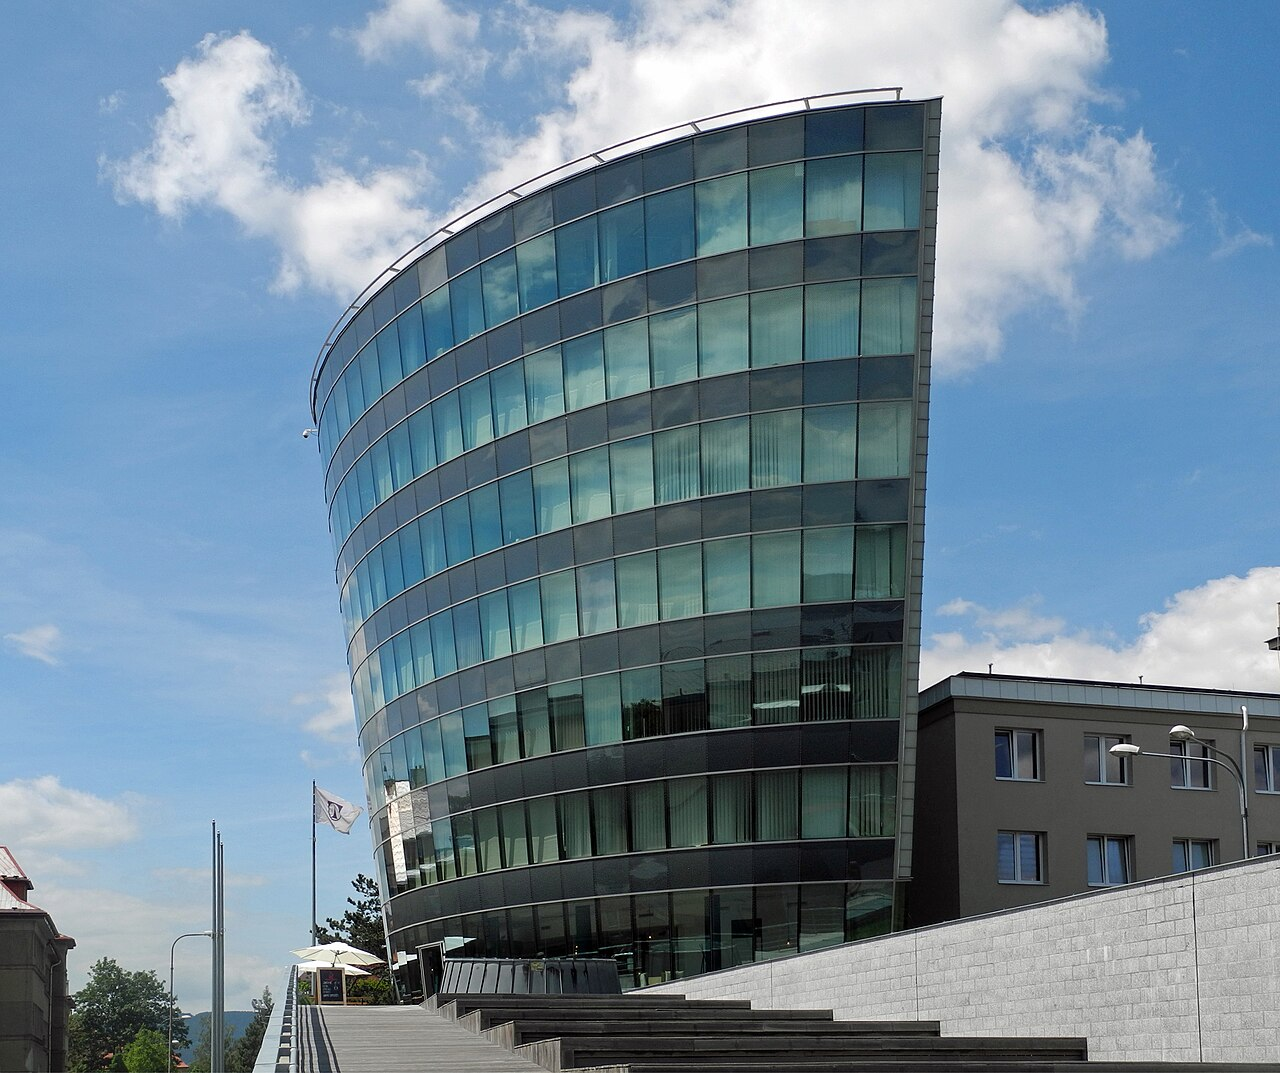
\includegraphics[width=0.5\linewidth]{pictures/Liberec-TUL-Rektorat-1.jpg}
  \caption{Nový rektorát a~informační centrum}
  \label{fig:tul-rektorat}
\end{figure}

\clearpage

Během následujících let se škola rozrůstala nejen o~nové studenty, ale také o~nové prostory: byly postaveny nové koleje, získána budova bývalé textilní továrny v~Doubí a~další budovy v~okolí dnešního Studentského náměstí. Roku 1958 dokončilo školu prvních 121 absolventů slavnostní promocí v~libereckém divadle. Roku 1960 byla škola rozdělena na~fakultu strojní a~textilní a~stala se z~ní \textit{Vysoká škola strojní a~textilní v~Liberci} (VŠST). Dále byly získány budovy v~Sokolské ulici (dnešní budova S), objekt po~zrušeném pedagogickém institutu v~Komenského ulici (budova P). S~nárůstem počtu studentů samozřejmě přestala stačit ubytovací kapacita tehdejších kolejí. Proto byla roku 1977 v~libereckém Starém Harcově zahájena výstavba komplexu šesti kolejních bloků o~kapacitě 2300 lůžek, nové menzy a~dalších zařízení. Komplex byl ve~své dnešní podobě dokončen roku 1990.~\cite{niznansky}

O~dva roky později (1992) byla získána budova bývalého Stavoprojektu ve~Voroněžské ulici (budova H) včetně dočasného sídla Investiční a~poštovní banky nově přestavěného na~univerzitní knihovnu. Ve~stejném roce získala škola také komplex ve~Vesci sloužící jako koleje a~laboratoře a~v~roce 1996 někdejší Dům politické výchovy na~třídě 1.~máje (budova K).~\cite{golka}

V~letech 1990--1994 zřídila škola další čtyři fakulty: pedagogickou v~roce 1990, hospodářskou (1992), architektury (1994) a~mechatroniky a~mezioborových inženýrských studií (1995). Díky takovému růstu, vlastní výzkumné činnosti a~zahraničním stykům byl škole zákonem č.~192/1994 Sb.\ z~27.~9.~1994 přiznán od~1.~ledna 1995 název \textit{Technická univerzita v~Liberci}.~\cite{zakon192}

\vspace{1.2em}
\begin{figure}[H]
  \centering
  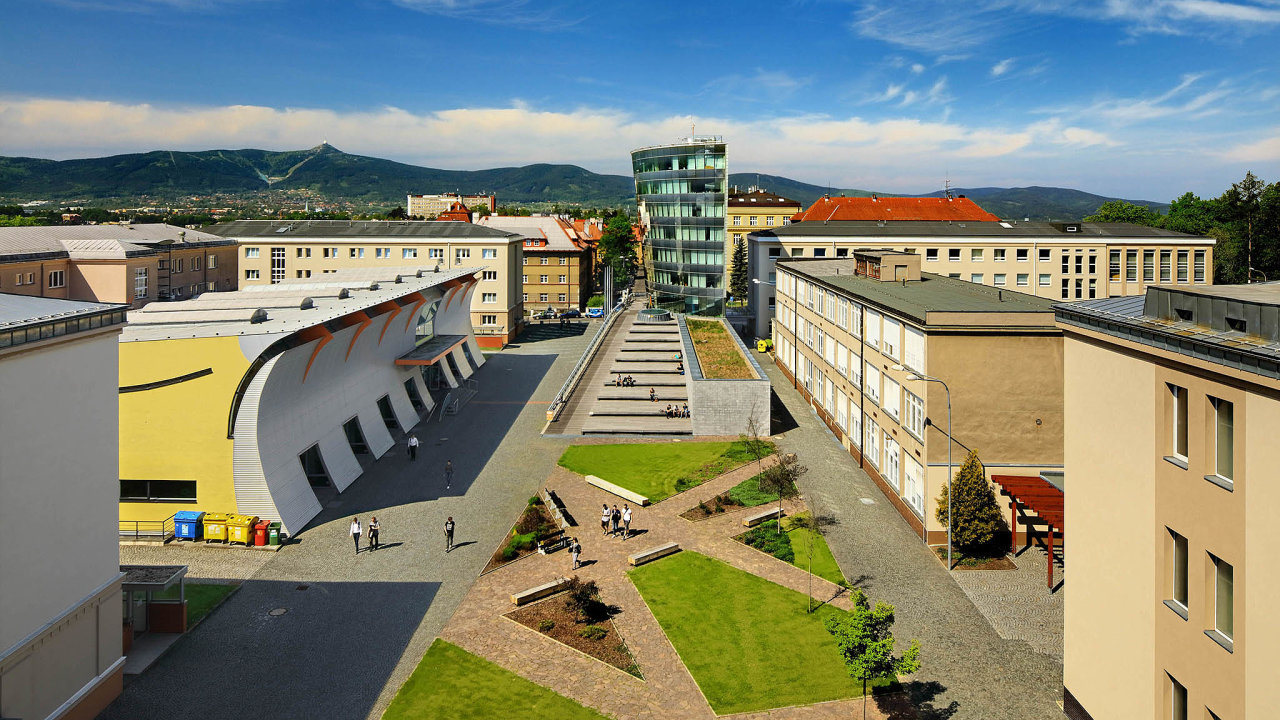
\includegraphics[width=0.6\linewidth]{pictures/kampus_tul.jpg}
  \caption{Kampus TUL, pohled z~budovy G}
  \label{fig:kampus-tul}
\end{figure}

\clearpage

\subsection{Rektoři Technické univerzity v~Liberci}

\begin{itemize*}
  \setlength{\itemsep}{-4pt}
  \item prof.\thinspace{}Ing.\thinspace{}Dr.\thinspace{}techn. Josef Kožoušek (1953--1961) % Doplněny úzké mezery v titulu
  \item doc.\thinspace{}Ing.\thinspace{}Vojtěch Dráb, CSc. (1961--1966) % Doplněny úzké mezery v titulu
  \item akad. Jovan Čirlič (1966--1969)
  \item prof.\thinspace{}Ing.\thinspace{}Jiří Mayer, DrSc. (1969--1973) % Doplněny úzké mezery v titulu
  \item akad. Jovan Čirlič (1973--1985)
  \item prof.\thinspace{}RNDr.\thinspace{}Bohuslav Stříž, DrSc. (1985--1990) % Doplněny úzké mezery v titulu
  \item prof.\thinspace{}Ing.\thinspace{}Zdeněk Kovář, CSc. (1990--1997) % Doplněny úzké mezery v titulu
  \item prof.\thinspace{}RNDr.\thinspace{}David Lukáš, CSc. (1997--2003) % Doplněny úzké mezery v titulu
  \item prof.\thinspace{}Ing.\thinspace{}Vojtěch Konopa, CSc. (2003--2010) % Doplněny úzké mezery v titulu
  \item prof.\thinspace{}Dr.\thinspace{}Ing.\thinspace{}Zdeněk Kůs (2010--2018) % Doplněny úzké mezery v titulu
  \item doc.\thinspace{}RNDr.\thinspace{}Miroslav Brzezina, CSc., dr.\thinspace{}h.\thinspace{}c. (od~roku 2018)~\cite{golka} % Doplněny úzké mezery v titulu
\end{itemize*}

\clearpage

\section{Fakulty a~univerzitní ústavy}

Univerzita má v~současnosti sedm fakult~\cite{golka,jandova}:
\begin{itemize*}
  \setlength{\itemsep}{-4pt}
  \item \textbf{Fakulta strojní}, založena 1953
  \item \textbf{Fakulta textilní}, založena 1960
  \item \textbf{Fakulta přírodovědně-humanitní a~pedagogická} (FPHP/FP), založena 1990 jako Fakulta pedagogická (FP), přejmenována 2008
  \item \textbf{Ekonomická fakulta} (EF), založena 1992 jako Hospodářská fakulta (HF), přejmenována 2009
  \item \textbf{Fakulta umění a~architektury} (FUA/FA), založena 1994 jako Fakulta architektury (FA), přejmenována 2007
  \item \textbf{Fakulta mechatroniky, informatiky a~mezioborových studií} (FMIMS/FM), založena 1995 jako Fakulta mechatroniky a~mezioborových inženýrských studií (FMMIS/FM), přejmenována 2008
  \item \textbf{Fakulta zdravotnických studií} (FZS), založena 2016, vznikla z~Ústavu zdravotnických studií (ÚZS), který byl založen v~roce 2004
\end{itemize*}

a~jeden univerzitní ústav:
\begin{itemize*}
  \setlength{\itemsep}{-4pt}
  \item \textbf{Ústav pro nanomateriály, pokročilé technologie a~inovace} (CxI), založen 2009
\end{itemize*}

\vspace{1em}
\begin{figure}[H]
  \centering
  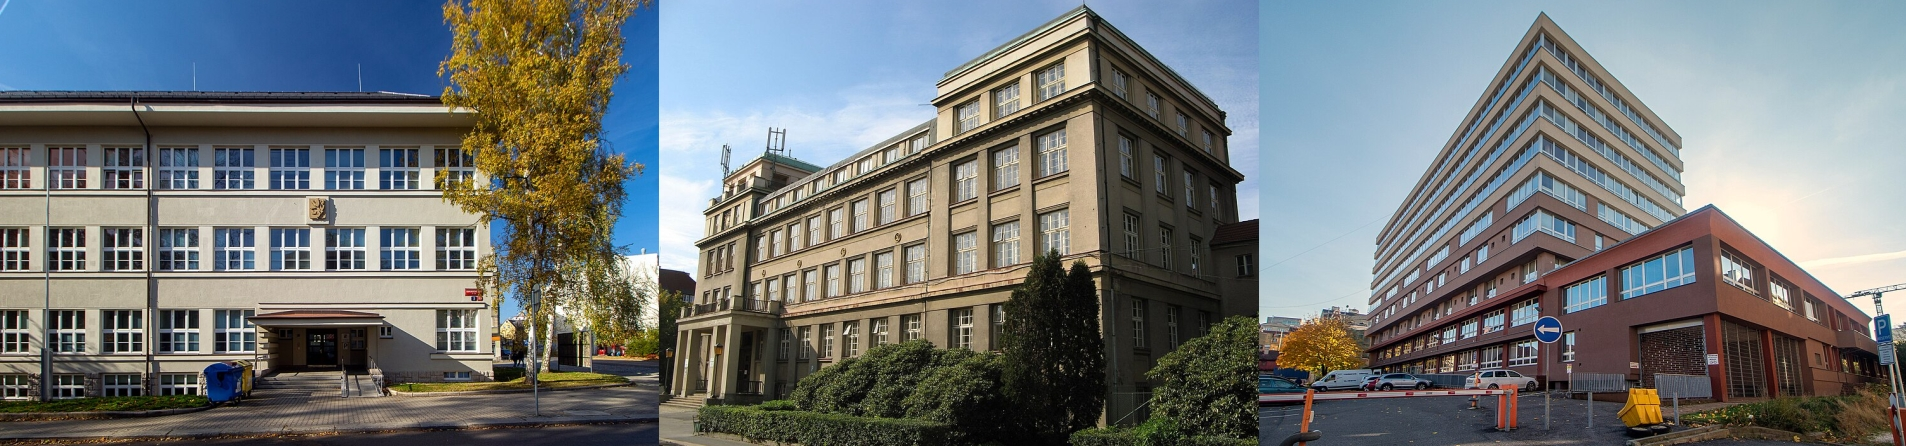
\includegraphics[width=0.9\linewidth]{pictures/budovy_p_b_t_tul.jpg}
  \caption{Budovy P (FP), B (FT) a~H (EF)}
  \label{fig:budovy-fp-ft-ef}
\end{figure}

Univerzita dále provozuje \textbf{Centrum dalšího vzdělávání} (CDV). Centrum organizuje řadu kurzů dalšího a~celoživotního vzdělávání, například kurzy pedagogické přípravy nebo jazykové kurzy. Zároveň CDV zajišťuje univerzitu třetího věku pro zájemce od~50\thinspace{}let.~\cite{jandova} % Doporučena úzká mezera za číslem

\clearpage

\section{Současnost TUL}

V~areálu Husova je menza, informační centrum, studentský klub, pobočka Univerzitní knihovny a~školka. Univerzitní školka „ŠkaTULka" je určena pro 48\thinspace{}dětí ve~věku od~3\thinspace{}let, kterým nabízí přístup Montessori a~Waldorfské pedagogiky.~\cite{jandova} % Doporučeny úzké mezery za čísly

O~životě na~Technické univerzitě v~Liberci informuje od~roku 2001 zpravodajský časopis \textit{T-UNI online}. Na~univerzitě dále působí řada studentských organizací včetně studentské unie.~\cite{jandova}

\subsection{Ubytování}

Studentské koleje jsou umístěny ve~Starém Harcově na~ulici 17.~listopadu 587/8. V~letech 2011, 2013 a~2014 zvítězily ve~studentské anketě „Kolej roku". Součástí areálu jsou dvě sportovní haly, tělocvičny, lezecká stěna, sauna, posilovna, minigolf, lanové centrum, fotbalové hřiště a~hřiště na~beach volejbal.~\cite{menzy}

\subsection{Dětská univerzita}

Od~roku 2008 probíhá na~TUL Dětská univerzita, celoroční volnočasové neformální vzdělávání dětí a~mládeže ve~věku od~6\thinspace{}do~19\thinspace{}let v~oborech: elektrotechnika, fyzika, přírodní vědy, strojírenství, textilní obory, robotika, programování a~matematika. Výuka kopíruje vysokoškolské studium včetně promoce, zápočtů a~zpracování závěrečné práce.
~\cite{jandova} % Doporučeny úzké mezery za čísly

\subsection{Sport}

O~sportoviště se stará Akademické sportovní centrum, které organizuje také fotbalovou, florbalovou, basketbalovou a~volejbalovou ligu. Na~TUL existuje Volejbalový klub a~Badmintonový klub, další z~nich se soustředí v~Univerzitním sportovním klubu Slavia.
~\cite{golka}

\clearpage

\subsection{Univerzitní sportovní klub Slavia Liberec}

Současný Univerzitní sportovní klub Slavia Liberec (USK Slavia Liberec) byl založen v~říjnu 1953 Jaroslavem Tyšlem jako Vysokoškolská tělovýchovná jednota Vysoké školy strojní (VŠTJ Slavia VŠS), která měla původně pět oddílů: odbíjená, basketbal, kopaná, lyžování a~lední hokej. Ke~31.~prosinci 2016 měl klub 255\thinspace{}členů v~osmi sportovních oddílech: basketbal, volejbal, lyžování, tenis (od~roku 1955), horolezectví (od~roku 1961), karate (od~roku 1977), futsal (od~roku 1994) a~florbal (od~roku 1995).~\cite{golka} % Doporučena úzká mezera za číslem

\clearpage

\section{Základní informace o~univerzitě}

\vspace{-0.6em}
\begin{table}[H]
\centering
\small
\begin{tabular}{ll}
\midrule
Název & Technická univerzita v~Liberci \\
Zkratka & TUL \\
Rok založení & 1953 \\
Typ školy & veřejná \\
Rektor & doc.\thinspace{}RNDr.\thinspace{}Miroslav Brzezina, CSc., dr.\thinspace{}h.\thinspace{}c. \\ % Doplněny úzké mezery v titulu
Kvestorka & Ing. Martina Froschová \\
Počet studentů bakalářského studia & 4230 \\
Počet studentů magisterského studia & 1419 \\
Počet studentů doktorského studia & 299 \\
Počet akademických pracovníků & 576 \\
Počet fakult & 7 \\
Sídlo & Liberec \\
Web & https://www.tul.cz \\
\bottomrule
\end{tabular}
\caption{Základní informace o~Technické univerzitě v~Liberci~\cite{vyrocnizprava}}
\label{tab:zakladni_informace}
\end{table}
\vspace{0.8em}

\section{Vedení univerzity}

\vspace{-0.6em}
\begin{table}[H]
\centering
\small
\begin{tabular}{ll}
\toprule
\textbf{Funkce} & \textbf{Jméno} \\
\midrule
Prorektor pro rozvoj & PhDr.\thinspace{}Ing.\thinspace{}arch.\thinspace{}Lenka Burgerová, Ph.D. \\
Prorektorka pro zahraniční vztahy & doc.\thinspace{}Ing.\thinspace{}Kateřina Maršíková, Ph.D. \\
Prorektor pro vědu a~výzkum & prof.\thinspace{}Dr.\thinspace{}Ing.\thinspace{}Petr Lenfeld \\
Prorektor pro informatiku & doc.\thinspace{}RNDr.\thinspace{}Pavel Satrapa, Ph.D. \\
Prorektor pro vzdělávání a~vnitřní legislativu & prof.\thinspace{}Ing.\thinspace{}Miroslav Žižka, Ph.D. \\
Předseda & doc.\thinspace{}Ing.\thinspace{}Vlastimil Hotař, Ph.D. \\
\bottomrule
\end{tabular}
\caption{Vedení Technické univerzity v~Liberci~\cite{vyrocnizprava}}
\label{tab:vedeni}
\end{table}

\clearpage

\custombibliography

\end{document}
